\section{编程与计算模型}
\label{sec:programming-model}
本节介绍 \SystemName{}如何通过一套声明式编程模型与运行时计算模型落实上述设计原则。

\begin{figure}[t]
\centering
\begin{lstlisting}[
    caption={\SystemName{} 的声明式编程模型。},
    label={list:api-example-1}
]
import rollart.distributed as rdist
from rdist.worker import AcrtorTrainCls, ActorGenCls, RewardCls
from rdist import ResourceManager as RM

class MyActorTrain(ActorTrainCls):
    @rdist.register(mode="execute_all")
    def compute_gradients(self, input_tensor):
        ...

gen_rm=RM({"H800": list(range(0, 8))},
          {"H20", list(range(8, 32))})

class HeteroActorGen(ActorGenCls):
    @rdist.hw_mapping(
      hw_affinity={"FrozenLake": "H800","default": "H20"}
    )
    def generate(self, input_ids, tag_name="default"):
        return self.model.process(prompt)

class ServerlessRewardWorker(RewardCls):
    @rdist.register_serverless(
        attribute='reward_proxy',
        serverless_url='fc://xxx.xxx')
    def compute_rewards(self, traj: list):
        prompt = f"Evaluate the trajectory:{traj}"
        return ray.get(self.reward_proxy(prompt))
\end{lstlisting}
\end{figure}

\subsection{声明式编程模型}
在 \SystemName{} 中，worker 是资源占有的最小单位。\autoref{list:api-example-1} 展示了其在 worker 函数层面的编程模型，这让运行时能够以细粒度感知资源使用方式。

\noindent\textbf{单控制器模型。}
工业界很多 RL 框架都采用单控制器模型~\cite{verl,slime_github}，因为它简化了 agentic RL 流水线的搭建。\SystemName{}也采用这一范式，并用 \texttt{register} 装饰器实现。当执行模式设置为 \texttt{execute\_all} 时，运行时会把输入广播给所有 trainer worker，并在各 worker 上调用 \texttt{compute\_gradients}。分布式计算与通信由系统负责，用户只需要在执行函数内部实现计算逻辑，再通过不同类型 worker 的函数组合整个训练流程。

\noindent\textbf{硬件亲和映射（原则 1）。}
\SystemName{}通过字典式资源描述支持异构资源组配置。以 \texttt{HeteroActorGen.generate} 为例，用户可借助 \texttt{hw\_mapping} 装饰器为某个 worker 方法声明细粒度硬件映射：被标记为 \texttt{FrozenLake} 的生成请求优先路由到 H800，其余请求优先进入 H20。函数参数 \texttt{tag\_name} 作为动态路由提示，使每次生成请求都能自动分配到绑定了合适硬件的 worker。这样，每条轨迹都能以最匹配的资源形态执行。

\noindent\textbf{无状态组件注册（原则 3）。}
用户可以通过 \texttt{register\_serverless} 装饰器，把奖励函数等无状态计算绑定到外部 serverless 接口。对用户而言，这与调用本地函数几乎一致；对系统而言，它意味着这部分计算不再占用常驻 GPU，而是可以利用外部平台进行弹性扩缩容。

\subsection{计算模型}
\PHM{轨迹级 rollout。}
\SystemName{}将单条轨迹视为 rollout 的核心执行单位。每个 \texttt{EnvManager} 维护一条或多条轨迹的状态机：先通过 \texttt{reset} 初始化环境，再进入事件循环，与共享的 \texttt{LLMProxy} 反复交互。环境将历史观测与动作序列送入 \texttt{LLMProxy} 生成下一步动作，再把动作应用到环境上，并记录新观测，直到轨迹结束。这种设计让不同轨迹彼此独立，避免批次级同步带来的等待。

\PHM{冗余环境 rollout。}
基于轨迹级设计，系统可以执行所谓\textit{冗余环境 rollout}：即启动多于理论所需数量的环境副本。一旦目标数量的轨迹已经收集完成，其余尚未结束的 rollout 可以直接终止。由于调度以轨迹为粒度，慢环境不会阻塞快环境，从而显著缓解 fail-slow 与 fail-stop 问题。论文实验表明，这一技术可以切实提升 rollout 效率。

\begin{figure}[t]
\centering
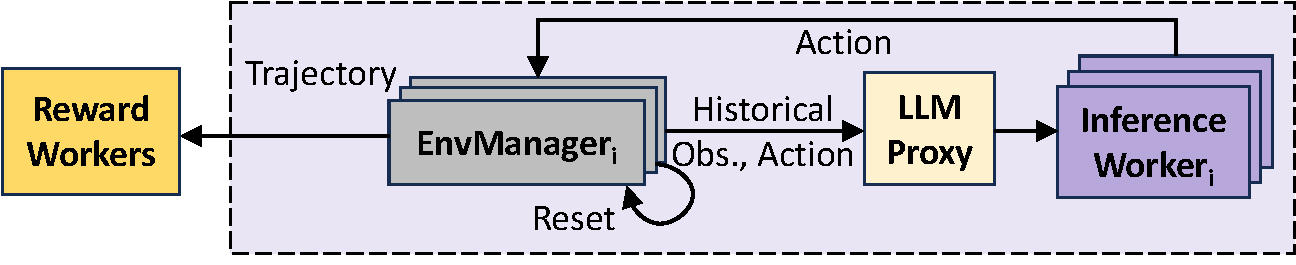
\includegraphics[width=\linewidth]{figs/overview/traj-level-rollout.pdf}
\caption{轨迹级 rollout 调度示意。}
\label{fig:traj_rollout}
\end{figure}

\PHM{异步训练工作流。}
\autoref{fig:rollout_scheduler} 展示了 \SystemName{} 如何编排异步训练流程。rollout 阶段中，多个 \texttt{EnvManager} 独立运行，持续生成轨迹并推入 \texttt{SampleBuffer}；推理 worker 与训练 worker 部署在不同 GPU 上，从而形成真正的解耦式训练。

训练阶段会周期性执行权重同步协议：先阻塞式调用 \texttt{get\_batch} 从 \texttt{SampleBuffer} 取出一批轨迹，再发出 \texttt{suspend} 暂停采样，随后拉取最新模型并把权重广播给所有推理 worker，最后通过 \texttt{resume} 恢复轨迹级 rollout。上一轮未完成的轨迹也可通过 KV cache 重算在下一轮继续利用。随后系统在已取出的数据上执行 \texttt{train\_step}。在异步模式下，training 与 rollout 相互重叠，而系统用异步边界控制轨迹的新鲜度。

\begin{figure}[t]
\centering
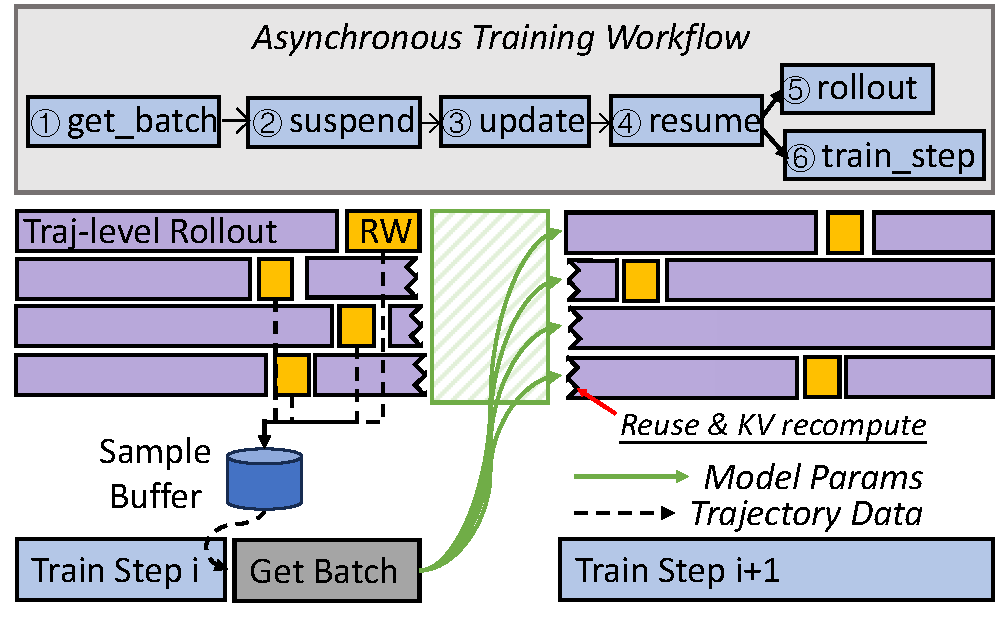
\includegraphics[width=\linewidth]{figs/overview/rollout_scheduler_osdi_resume.pdf}
\caption{异步训练工作流。}
\label{fig:rollout_scheduler}
\end{figure}

\PHM{异步边界。}
异步训练允许轨迹在旧版本模型下开始生成、在更新后的新模型下继续执行，因此一批轨迹中可能混杂多个模型版本。样本陈旧性会提高方差并损害稳定性。AReaL~\cite{areal} 用平均样本新鲜度做约束；\SystemName{}则引入每轨迹的\textbf{异步边界} $\alpha$，定义为当前 agent LLM 版本与该轨迹启动版本之间允许的最大差值。若模型已推进到版本 $n$，则 \texttt{SampleBuffer} 中任何轨迹都必须由不早于 $(n-\alpha)$ 的版本启动；超出该约束的轨迹将被中止。论文实验显示，$\alpha=1$ 通常能在训练速度和稳定性之间取得较优平衡。
